% \begin{figure}[h]
% \centering
% \includegraphics[scale=0.5]{graph_a}
% \caption{An example graph}
% \label{fig:x cubed graph}
% \end{figure}

\documentclass[
% twoside,
fontsize=12pt,
paper=a4,
abstract=true,
listof=totoc,
headings=standardclasses,
chapterprefix=false,
numbers=noenddot,
parskip=half+, % comment this out if you do not want an empty half line between paragraphs, but please read the KomaScript Guide and search for parskip (around page 82): ftp://ftp.dante.de/pub/tex/macros/latex/contrib/koma-script/scrguide.pdf
]{scrreport}

\usepackage{enumitem}
\usepackage{varwidth}
\usepackage{tasks}

\usepackage{listings} %source code listings
\lstdefinestyle{mystyle}{
    basicstyle=\ttfamily\footnotesize,
    % breakatwhitespace=false,         
    % breaklines=true,                 
    captionpos=b,                    
    % keepspaces=true,                 
    % numbers=left,                    
    % numbersep=5pt,                  
    % showspaces=false,                
    % showstringspaces=false,
    % showtabs=false,                  
    % tabsize=2
}

\lstset{style=mystyle}

\usepackage[utf8]{inputenc} 
\usepackage{graphicx}
\graphicspath{ {./img/} }
\usepackage{amsmath}
\usepackage{amssymb}
\usepackage{amsthm}
\theoremstyle{definition}
\newtheorem{definition}{Definition}%[chapter]
\theoremstyle{remark}
\newtheorem{remark}{Remark}

\usepackage{float}
\usepackage[normalem]{ulem}
\usepackage[automake,acronym, toc]{glossaries}
\makeglossaries
\loadglsentries{glossary.tex}
\usepackage{hyperref}
\hypersetup{
    pdftitle={Standards Based Personal Knowledge Graphs},    % title
    pdfauthor={Omes Baltes},
    linktoc=all,
    colorlinks=true,       % false: boxed links; true: colored links
    linkcolor=black,       % color of internal links (change box color with linkbordercolor)
    citecolor=blue,       % color of links to bibliography
    urlcolor=cyan       % color of external links
}
\usepackage[
backend=biber,
style=ieee,
sorting=nyt
]{biblatex}
% \PassOptionsToPackage{hyphens}{url}
\addbibresource{references.bib} %Import the bibliography file

\renewcommand\lstlistlistingname{List of Code}

%%%%%%%%%%%%%%%%%%%%%%%%%%%%%%%%%%%%%%%%%%%
% Preamble
%%%%%%%%%%%%%%%%%%%%%%%%%%%%%%%%%%%%%%%%%%%
\title{Standards Based Personal Knowledge Graphs}
\author{Omes Felix Baltes}
\date{15. July 2022}

\begin{document} % you have to do this to start the document
\begin{titlepage}
    \begin{center}
        \vspace*{1cm}
        \Huge
        Standards Based Personal\\ Knowledge Graphs \\
        
        \vspace*{1cm}
        
        \Large
        Omes Baltes
      
        \vfill

        \large
        Bachelor's Thesis -- 15. July, 2022\\
        Ruhr University Bochum\\
        Faculty of Mathematics\\
        \vspace{1cm}

        \begin{itemize}[noitemsep, leftmargin=13.9em]
            \item[Supervisor:] Prof. Maribel Acosta 
            \item[Advisor:] Prof. Ajsa Fischer
        \end{itemize}
        
        % Supervisor: Prof. Maribel Acosta \\
        % Advisor: Prof. Ajsa Fischer
        
    \end{center}
\end{titlepage}
\pagenumbering{roman}
\vspace*{\fill}

\begin{center}
© 2022\\
Omes Baltes\\
ALL RIGHTS RESERVED
\end{center}
\thispagestyle{empty}
\begin{abstract}
\thispagestyle{plain}
Personal knowledge graphs as the foundation for personal knowledge management have gained increasing attention from the industry. The tools associated with these terms are based on proprietary technologies, resulting in vendor lock-in and limited functionality. This thesis explores how personal knowledge graphs can leverage open semantic web standards to increase their expressiveness, interoperability and capabilities.
\end{abstract} 
\begin{center}
    
\vspace*{4cm}
My gratitude goes to 

Prof. Acosta for the space to grow \\
Sebastian for the paths to wander \\
Hendrik \& Lara for the company on the way
\end{center}

\tableofcontents


%%%%%%%%%%%%%%%%%%%%%%%%%%%%%%%%%%%%%%%%%%%
% Chapters
%%%%%%%%%%%%%%%%%%%%%%%%%%%%%%%%%%%%%%%%%%%
\chapter{Introduction} \label{ch:introduction}
\pagenumbering{arabic}
The never-ending growth of data and information is overwhelming the natural capacities of the human brain. This phenomenon is known as the information overload problem. Personal Knowledge Graphs (PKGs) have recently garnered increasing attention from the industry as a promising solution to information overload on the individual level. The need for Individuals to structure and organize sources of knowledge has long been recognized. Over the last decades, a multitude of productivity tools have been developed to augment the abilities of the human mind. Applications for text processing, file and task management, vocabulary training, note-taking, and mind-mapping, all try to help humans manage the information and knowledge at their disposal. 

% Personal Knowledge Graphs (PKGs) have recently garnered increasing attention from the Industry. Encompassing concepts from Knowledge Graphs (KGs), Personal Knowledge Management (PKM) and Intelligence Amplification, PKGs are a promising approach to the information overload problem on the individual level. Information overload is caused by the never-ending growth of Data and Information overwhelming the natural capacities of the human brain. The need for Individuals to structure and organize these sources of knowledge has been recognized. Over the last decades, a multitude of productivity tools have been developed to augment the abilities of the human mind. Applications for text processing, file and task management, vocabulary training, note-taking, and mind-mapping, all try to help humans manage the information and knowledge at their disposal. 

In more recent years there has been a wave of tools focusing on the need to have all of this knowledge centralized and interlinked. This freely associative approach to knowledge is supposed to mimic the way humans think. Some of these tools take this as motivation to market themselves as “Tools for Thought”, claiming to enable maintenance of a lifelong “Second Brain”, “Personal Knowledge Graph”, or “Digital Garden”.

In Research, PKGs are a mostly uncharted area, based on Knowledge Graphs (KGs), and associated with Personal Knowledge Management (PKM) and Intelligence Amplification. As even the definition of Knowledge Graphs is contentious, PKGs are not clearly defined yet. In broad terms, PKGs are data graphs of structured Knowledge that is relevant or related to the person in question. The Notion of a PKG is an evolving concept that combines ideas from Computer Science, Information Science, Data Science, Mathematics, Psychology and Philosophy. The focus of this thesis is on the practical implications of PKGs serving as the foundation for Personal Knowledge Management.

\section{Vision}
% avoid talking down to your readers
The vision of personal knowledge management based on PKGs can be realized by building a PKG Ecosystem. This ecosystem would consist of a data model for PKGs and all the tools and technologies that interact with it. To motivate this idea, we present examples of how the PKG Ecosystem might impact the way we interact with information, knowledge and technology. We hope this will develop an understanding for the importance of this technology, and the paradigm shifts it can enable, as well as provoke thoughts on the status quo of data ownership in technology. Consider the following examples:

\textbf{Data centralization, ownership and binding.} \sout{Imagine} after changing your address you just have to update the address in one place: Your PKG. From this point onwards, anyone you shared your address with previously, will automatically retrieve the most up-to-date address. In your PKG tool, you can always see who has access to your information and revoke it at any time. Contrast this with the current situation of having to update a copy of your address across dozens of external data silos which you have limited control over.

\textbf{Free association of knowledge.} \sout{Imagine} you are visiting a Wedding in Spain with some wonderful people and dancing to a Song. In a PKG you can freely associate/link all of this information, just like your brain does. You then have multiple associative retrieval paths to remember the song, because it is connected to the people, the wedding, the location and the Spain trip. You can also freely associate any information with the song, for example, make notes, which is not possible on \gls{vendorlockin}ed data, that is coupled with the app, like Spotify.

\textbf{Transclusion and bi-directional links.} \sout{Imagine} you have a file or website that you frequently quote from. Traditionally you would copy and paste the content, and have duplicates all over your workspace, without necessarily knowing where the information came from. In your PKG you can attach links to this information, specifying the location of the original. If the link is a pointer within your PKG, you can even update the content in any location and it will prompt you, asking if you want to update it in all other locations in real-time. Information in your PKG that is linked towards will show the locations referencing it.

% \textbf{Integrating external Data.} There are many browser extensions for saving and organizing bookmarks. Saving things should be as easy as clicking a button on any kind of information, be it a Term in a dictionary, a Book, an Article, or a Movie. In contrast to just saving the URL, a PKG would give the option to save structured Data about this Object, like Information about the author, who recommended it, etc.

% better title?
\section{Current Limitations}
The increasing difficulty of Personal Knowledge Management was already identified early in the 20th century \cite{Bush1945Memex, Engelbart1962AHI}. The suggested approaches at the time were hindered by unsurmountable technological hurdles, which have all but disappeared by now \cite{Davies2005Memex60}. Still, even today's Tools for PKM are not powerful enough to address information overload. Even worse, these tools have limitations that make them unfit candidates for lifelong Personal Knowledge Management:

    \textbf{Proprietary technology and vendor lock-in.} They are based on proprietary technology. This causes vendor lock-in, which means the data stored can not be used in other tools without considerable switching costs. The user's data is sometimes even stored in data silos, meaning they do not have control over their data.

    \textbf{Lack of structure and expressivity.} They are based on unstructured plain text and do not support structured knowledge, schema or semantics. This means integrating or collaborating with external knowledge is not possible. These characteristics have proven indispensable for Knowledge Management in Industry and Academics, however. 
    
    \textbf{Query and search algorithms.} A direct consequence of the previous points. Only structured information, like data stored in databases, supports query languages. These tools do not support query languages and rely on rolling their own search algorithms. This limits them to a single Information retrieval path: full-text search, with the user required to remember the exact keywords of what they are looking for.
    
    \textbf{Lack of open standards} Even though these tools want to enable lifelong Personal Knowledge Management, they are not based on open standards. Interoperability with other data formats and services is not guaranteed. User's data might not be portable to other formats if the tool shuts down.

Open Standards for semantic Knowledge Graphs, called Semantic Web Technologies, are developed by the W3C. Theoretically, one could use Tools for Semantic Web Technologies to create PKGs and solve most of these limitations. Unfortunately, the tools based on Semantic Web Standards (SWSs) are notoriously hard to understand and use, even for computer scientist and programmers \cite{EasierRDF}. Expecting non-technical users to manage their personal knowledge with them is unrealistic.

% be a little be more descriptive about your approach in the introduction. What makes it special so that the reader wants to read about it
\section{Approach}
To address the problems and limitations outlined in this chapter, we embrace the vision of a PKG Ecosystem. We establish that the creation of such an ecosystem is possible and beneficial, by outlining its structure and \sout{desirable features} scope. We argue that the data model for PKGs should be a data graph based on Semantic Web Technologies. Such a data model is developed and described in detail. Applications implementing the model will benefit from all the features developed for the Semantic Web. They will be able to express semantics, use external schema, and reasoning and have support for mature query languages. 

Finally, we develop a prototypical implementation of the data model in the form of an interactive web application.

% It is important to keep a data-centric approach in mind when talking about PKGs, as they should serve as the foundation for lifelong personal knowledge management. Even advances in technology like Computer-Brain Interfaces and Artificial Intelligence should not render PKGs obsolete.

% \section{Structure}
% The thesis is structured as follows.
% \begin{description}
%     \item[Chapter \ref{ch:preliminaries}] defines concepts used throughout the thesis.
%     \item[Chapter \ref{ch:relatedwork}] explores the scientific context of this work.
%     \item[Chapter \ref{ch:ecosystem}] 
%     \item[Chapter \ref{ch:model}]
%     \item[Chapter \ref{ch:markdown}]
%     \item[Chapter \ref{ch:prototype}]
%     \item[Chapter \ref{ch:conclusions}]
% \end{description}

% For explanations of commonly used terms please refer to the glossary
% In chapter [Preliminaries] we go over basic terms used in the thesis. Chapter [PKG Ecosystem] analyses what an Ecosystem of Applications for PKGs needs to be capable of and compares it to current Personal Knowledge Management Tools. Chapter [PKG Model] presents a directed labeled Graph Data Model for PKGs based on SWS. This model is compatible with both text and databases. Chapter [Semantic Markdown] will explore an RDF extension to Markdown, to enable freely mixing structured and unstructured Information. In Chapter [UX POC] we present a proof of concept for an application that uses the proposed model and is focused on usability; requiring no technical expertise.
\chapter{Preliminaries} \label{ch:preliminaries}
This chapter provides definitions for concepts used throughout the thesis. For descriptions of terms and phrases please refer to the glossary.

\begin{itemize}
    \item Knowledge base
    \item knowledg graph 
    \item RDF 
    \item TURTLE
\end{itemize}

\begin{definition}[Graph]
    A \textbf{graph} is a tuple $G = (V, E)$, where $V$ is a set of \textbf{vertices} and $\displaystyle E\subseteq \{\{x,y\}\mid x,y\in V\;{\textrm {and}}\;x\neq y\}$ is a set of \textbf{edges}.
\end{definition}

\begin{definition}[Directed graph]
    A \textbf{directed graph} is a tuple $G = (V,E)$, where $V$ is a set of vertices and $\displaystyle E\subseteq \left\{(x,y)\mid (x,y)\in V^{2}\;{\textrm {and}}\;x\neq y\right\}$ is a set of \textbf{directed edges}.
\end{definition}

\begin{definition}[Labeled graphs]
    An \textbf{edge-labeled graph} is a graph that has a labelling function $l_E : E \rightarrow X$, where $X$ is a set of edge labels.
    A \textbf{vertex-labeled graph} is a graph that has a labelling function $l_V : V \rightarrow Y$, where $Y$ is a set of vertex labels.
    A \textbf{labeled graph} is a graph that is both edge-labeled and vertex-labeled.
\end{definition}

\begin{definition}[Multigraph]
    A \textbf{multigraph} is a tuple $\displaystyle G=(V,E,\phi )$, where $V$ is a set of vertices, $E$ is a set of edges and $\displaystyle \phi :E\to \{\{x,y\}\mid x,y\in V\;{\textrm {and}}\;x\neq y\}$ is an incidence function mapping every edge to an unordered pair of vertices.
\end{definition}

\begin{remark}
    These definitions can be combined to get a directed labeled multigraph.
\end{remark}


% \includegraphics[width=0.7\textwidth]{defKG.png}
% \begin{definition}[Knowledge Graph]
%     A \textbf{Knowledge Graph} is a directed labeled multigraph.
% \end{definition}

\begin{remark}
    The definition of a KG remains contentious \cite{Hogan2021KG,commonsenseKG}.
\end{remark}

\begin{figure}[H]
    \centering
    \includegraphics[width=0.5\textwidth]{kg}
    \caption[]{A Knowledge Graph}
\end{figure}

\begin{figure}[H]
    \centering
    \includegraphics[width=0.75\textwidth]{rdf}
    \caption[]{An RDF Graph}
\end{figure}

% For more background on these concepts, we refer the reader to the primer on the subject by Hogan et al \cite{Hogan2021KG} and the official W3C specifications \cite{rdf, rdfs, owl, turtle, sparql, xsd}.

% comment: This is not an RDF graph. 

% This picture is not correct in several ways: 

% 1. In an RDF triple, properties are labels of the edges, not nodes themselves. So, in the RDF triple (Q9439, P22, Q157009) P22 is just the label of the edge, not a node. This also solves the problem that some of your edges do not have labels, which is not allowed in RDF. 

% 2. The labels for properties like label_en and label_de is not the standard way of representing human-readable labels in RDF. For that we use rdfs:label, and it is ONE property, without distinction of the the language in the property. If you want to say that the value is in a specific language, then we use language-tagged literals … for example “Queen Victoria”@en. 

% 3. It is a convention when plotting RDF graphs to use rectangles for depicting  literals, and ovals for IRIS 
\chapter{Related Work} \label{ch:relatedwork}

A search in academic search engines yields about a dozen results with "Personal Knowledge Graph" in the title. They are a novel research area. We observed different perceptions of PKGs in related work, depending on the perspective and context of the authors. These perceptions can roughly be grouped into the following categories:

\textbf{PKGs as special cases of knowledge graphs.} Here PKGs are conceived as KGs about an individual, or personalized KGs. The focus lies on knowledge "about" the person and its relationships to other entities. This knowledge could for example be used by digital personal assistants to great effect. The PKG is mostly generated and maintained without intervention by the user.

\textbf{PKGs as the basis for personal knowledge management.} The focus lies on knowledge "relevant" to the person. The knowledge is in part generated and maintained by the user. Tools for interacting with PKGs are a logical consequence.

In the following sections, we will look at related work in each of these categories.

\section{Knowledge Graphs}

Hogan et al provide a comprehensive overview of knowledge graphs and related concepts and technologies \cite{Hogan2021KG}. They notably only distinguish two types of knowledge graphs in practice: open knowledge graphs and enterprise knowledge graphs. They explain that consensus-based schema, identity and context play a key role for knowledge graphs. If PKGs were implemented the same as the knowledge graphs described by Hogan et al, everything covered in their paper would also apply to them. In contrast to open and enterprise KGs, however, PKGs will probably not be maintained by large organizations or communities. This is an important difference to keep in mind, because it will likely result in schemas and contexts, that are not consensus-based and thus less expressive, harder to merge and not in line with linked open data principles.

Balog and Kenter established PKGs as a research area with their research agenda \cite{Balog2019PKGAgenda}. They define PKGs as "a source of structured knowledge about entities and the relation between them, where the entities and the relations between them are of personal, rather than general, importance. The graph has a particular “spiderweb” layout, where every node in the graph is connected to one central node: the user". They differentiate general KGs from PKGs by stating that KGs concern public or global entities. This rules out non-public entities that individuals might find relevant for their PKGs. Their definition is quite broad, but we would like for it to not enforce a "spiderweb" layout and also include entities that are just relevant and not related to the user. Broadening the definition in this way would connect the perceptions of PKGs about an individual and PKGs for personal knowledge management.

Safavi et al describe a methodology to summarize KGs personalized to the users' interest \cite{Safavi2019PKGSum}. This highlights other differences between PKGs and KGs: Data in a PKG should be relevant to its user, and it should focus on being human readable. Many KGs are primarily composed of knowledge relevant to machines.
    

\section{Personal Knowledge Management}
Bush wrote about his vision of the Memex, an external device acting as a  supplement to an individual's memory \cite{Bush1945Memex}. This vision was held back by technical limitations at the time, but highly influential. Davies et al were motivated by this vision and wrote about personal knowledge bases 60 years later, noting that the technical hurdles were gone and suggesting semantic web technologies, which were new at the time, as a promising approach. \cite{Davies2005Memex60}. These papers were highly influential to this thesis. Even though the terms have changed from "memex" and "personal knowledge base" to "second brain", "personal knowledge graph" etc., their vision remains in large parts intact and unfulfilled as discussed in this thesis.

Velitchkov writes about ontologies for his PKM tool Roam Research \cite{roamOntologies}. He emphasizes that ontologies for personal knowledge graphs are important and beneficial.

Matuschak writes about the limitations of text and books and analyses the difficulty of building intelligence augmenting tools for thought \cite{Matuschak2019TTFT}.

\section{PKG Tools}

As mentioned in chapter \ref{ch:introduction}, several tools associate themselves with PKGs. The most relevant ones at the time of writing are Notion, Obsidian, Roam Research, LogSeq and RemNote \cite{notion, roam, obsidian, logseq, remnote}. These tools will be discussed in chapter \ref{ch:ecosystem}.
\chapter{PKG Ecosystem} \label{ch:ecosystem}

Kickstarting the development of a PKG ecosystems is a prerequisite for realizing the vision of PKGs. The PKG ecosystem would consist of all the technologies, protocols and models that enable individuals to interact with their PKGs. Apart from enabling personal knowledge management, a PKG ecosystem could also address other problems in our technology landscape. Concerns about data silos, vendor lock-in and privacy are increasingly brought up in research and politics \cite{missingCitation}. Considering the examples in chapter \ref{ch:introduction} we believe a PKG ecosystem is a promising approach to these problems.

We group the PKG ecosystem into three areas, like tech stacks in the industry:
% include a figure of this structure

\begin{itemize}
    \item Data model
    \item Backend and Protocols
    \item Applications
\end{itemize}

Data and storage models will be discussed in chapter \ref{ch:model}.

The backend will have the typical responsibilities of a backend server for modern applications. It will store an implementation of the data model, provide protocols for accessing the data, handle requests, manage access rights, etc.
We will only describe functionalities expected from this backend, the implementation will not be a part of this thesis.

Once the data model and backend exist, they will provide a software platform that developers can target with their applications. For applications to work consistently across backends provided by different vendors, it would be beneficial for the data model and protocols to be open standards.
We present a prototype of an application like this in chapter \ref{ch:prototype}.

The PKG ecosystem is a large-scale undertaking similar in complexity to online cloud services. In this chapter, we analyze required functionalities this ecosystem needs to be capable of and compare it with the current software lanscape of personal knowledge management tools.

% It was noted that Knowledge Graphs can be considered, more than a precise notion or system, an evolving project, and a vision \cite{KGHistory}. The same applies to PKGs. This evolving project is composed of requirements identified in Personal Knowledge Management over the last decades. The Term PKG ecosystem encompasses PKGs, Tools that work with them, and the entire Tech Stack that enables both to function. 

% Before considering the Data and Storage Models underlying a PKG, there needs to be a clear understanding of what the PKG Ecosystem needs to be capable of. We need to consider these feature requirements from the outset; otherwise, the designed model might be unfit for the tasks ahead.

%%%%%%%%%%%%%%%%%%%%%%%%%%%%%%%%%%%%%%%%%%%%%%%%%%%%%%%%%%%%%%%%%%%%%%%%%%%%%%%%
\section{Functionalities}
%%%%%%%%%%%%%%%%%%%%%%%%%%%%%%%%%%%%%%%%%%%%%%%%%%%%%%%%%%%%%%%%%%%%%%%%%%%%%%%%

To gather the requirements for the PKG ecosystem, we assembled ideas present in research and industry \cite{Bush1945Memex, Davies2005Memex60, Matuschak2019TTFT,jones2007PIM}. Some of these ideas are already established and implemented across products. Others are theoretical or might even pose to be major implementation hurdles. Nonetheless, all of them are possible to implement with current technological capabilities.

For each of the proposed categories, we list the essential ideas that we deem requirements for the successful development of a PKG ecosystem.

%%%%%%%%%%%%%%%%%%%%%%%%%%%%%%%%%%%%%%%%%%%%%%%%%%%%%%%%%%%%%%%%%%%%%%%%%%%%%%%%
\subsubsection*{Data model}
%%%%%%%%%%%%%%%%%%%%%%%%%%%%%%%%%%%%%%%%%%%%%%%%%%%%%%%%%%%%%%%%%%%%%%%%%%%%%%%%

\textbf{Centralization.} All of the data in a PKG needs to be accessible in one place. This approach corresponds to a trend in operating systems search engines. Originally files, mails, calendars, bookmarks, and notes were coupled with their apps data silos and search. The modern approach is to have a single quick search that accesses data from all types of apps present on your PC, providing a centralized retrieval path.

\textbf{Free association of knowledge elements.} Our brain is able to freely associate any thought, without worrying about the type, category or hierarchy. We can associate the song we hear at a wedding, with the people, location, dance and food. Technology we use today, creates artificial partitions on our knowledge because it is stored in data silos. Interoperability is hindered by vendor lock-in. We are unable to connect our media, contacts, location and calendars. This limits our ability to associatively organize and express knowledge, and the number of paths available to retrieve it.

\textbf{Knowledge types and semantics.} A PKG needs to be able to store structured, semi- and unstructured Knowledge. Unstructured knowledge is data without metadata, e.g., text or images. Semi-structured knowledge includes metadata and structured knowledge is typed and based on schemata, e.g., database entities. Unstructured knowledge is quickly generated, like  a "thoughtsream" captured as a note or voice memo. Structured knowledge takes time to generate, organize and enrich, because types and schmema need to be considered for every entity. 

\textbf{Transclusion.} Also known as embeds or components, transclusion describes the ability for the same data to appear in several places. This is enabled by including data by reference, rather than duplicating it. For example, transclusion enables multiple documents that use the same paragraph to be updated as soon as the paragragh is changed in any location. It is a very powerful concept, that is barely used by non-technical people, where copy and pasting data is the norm.

\textbf{Based on open standards.} A PKG data model based on open standards provides portability and interoperability. We argue this is essential for knowledge work because it enables integrating and extracting data from diverse data sources.

%%%%%%%%%%%%%%%%%%%%%%%%%%%%%%%%%%%%%%%%%%%%%%%%%%%%%%%%%%%%%%%%%%%%%%%%%%%%%%%%
\subsubsection*{Applications}
%%%%%%%%%%%%%%%%%%%%%%%%%%%%%%%%%%%%%%%%%%%%%%%%%%%%%%%%%%%%%%%%%%%%%%%%%%%%%%%%
These requirements apply to applications for personal knowledge management. 
% For unstructured Information a frictionless thought capture process that does not interrupt the flow of ideas, is essential. Allowing Knowledge to be quickly captured as a Thoughtstream uninterrupted by prompts to structure it is essential for productive thinking.

\textbf{Text editing.} PKG tools need to allow free text processing. As we will see in the next section, all current PKG Tools include either a plain text markdown editor, an outliner markdown editor, or a WYSIWYG text processor.

\textbf{Views and filters.} PKGs will potentially store massive amounts of knowledge, so apps working with them need to provide filters to limit the complexity and volume of data shown. Different visualizations like interactive graphs, tables, galleries, and boards aided by filters can be used to present and navigate relevant information in a digestible way.

\textbf{Flexible refactoring.} changes of any magnitude to the schema, entities, relationships, and views in a PKG need to be frictionless and quick. This allows smooth refactoring of unstructured Knowledge into structured Knowledge.

\textbf{External knowledge.} Apps should provide features for integrating external knowledge. Structured external knowledge should be searchable and queryable. For semi- and unstructured knowledge, source capture and transclusion are considerations. When importing external knowledge, prompts and filters should be available to filter relevant knowledge.
    
\textbf{Bi-directional Links} The internet enables unidirectional links between websites. With bi-directional links, any site would show all sites that link to it. They have not been included, due to vandalism concerns. For moderated networks like wikis or personal knowledge graphs, vandalism is not a concern and bi-directional links are established as useful features.

%%%%%%%%%%%%%%%%%%%%%%%%%%%%%%%%%%%%%%%%%%%%%%%%%%%%%%%%%%%%%%%%%%%%%%%%%%%%%%%%
\subsubsection*{Backend}
%%%%%%%%%%%%%%%%%%%%%%%%%%%%%%%%%%%%%%%%%%%%%%%%%%%%%%%%%%%%%%%%%%%%%%%%%%%%%%%%
The requirements for the backend are similar to the backends in use today.

\textbf{Multiplatform Sync} PKGs should be available on any platform and sync changes between devices.

\textbf{Cloud Drive for Files} Most current PKM tools only allow for import and export of files. Editing, annotating or opening the files in other programs is not possible, which is a severe limitation. A PKG needs to provide or integrate with a cloud drive to access and edit files in real-time. This way files can also be freely associated with other data in the PKG.

\textbf{Version History} changes need to be backed up and reversible.

\textbf{Protocols and APIs} The backend should be compliant with protocols that enable access and querying of the storage model.







%%%%%%%%%%%%%%%%%%%%%%%%%%%%%%%%%%%%%%%%%%%%%%%%%%%%%%%%%%%%%%%%%%%%%%%%%%%%%%%%
\section{PKM Tool Software landscape}
%%%%%%%%%%%%%%%%%%%%%%%%%%%%%%%%%%%%%%%%%%%%%%%%%%%%%%%%%%%%%%%%%%%%%%%%%%%%%%%%

In this section, we provide a detailed comparison of select current personal knowledge management tools. We have looked at more than 50 tools and selected the most mature tools associated with PKGs \cite{notion, obsidian, roam, logseq, remnote}. We provide tables outlining the properties of these tools and analyze them in light of the requirements and limitations outlined previously.

\begin{table}[H]
    \centering
    \includegraphics[width=\textwidth]{fm01overview.png}
    \caption{PKM tool overview -- the software landscape}
    \label{fig:fm01overview}
\end{table}

Figure \ref{fig:fm01overview} shows a general overview of the software landscape. We can see that all of these tools are based on proprietary data formats. Most of them store data in the cloud to enable features like multi-platform sync and collaboration.


\begin{table}[H]
    \centering
    \includegraphics[width=\textwidth]{fm02workflows.png}
    \caption{PKM tool workflows -- what they can be used for}
    \label{fig:fm02workflows}
\end{table}

Figure \ref{fig:fm02workflows} shows the workflows these tools enable. Most of the tools allow task management and journaling. features like password protected pages and flash cards are only supported by a select few. Notably, only Notion includes databases with views and filters.

\begin{table}[H]
    \centering
    \includegraphics[width=\textwidth]{fm03editing.png}
    \caption{PKM tool editing -- text processing capabilities}
    \label{fig:fm03editing}
\end{table}

Figure \ref{fig:fm03editing} shows the text editing capabilities of the different tools.


\begin{table}[H]
    \centering
    \includegraphics[width=\textwidth]{fm04formats.png}
    \caption{PKM tool linking -- relationships between knowledge elements}
    \label{fig:fm04formats}
\end{table}

Figure \ref{fig:fm04formats} shows how the tools manage the granularity of their pages / blocks / entities and links between them. this concept is explained in more detail in chapter \ref{ch:model}.


\begin{table}[H]
    \centering
    \includegraphics[width=\textwidth]{fm05relationships.png}
    \caption{PKM tool formats -- interoperability with file formats}
    \label{fig:fm05relationships}
\end{table}

Figure \ref{fig:fm05relationships} shows the different file formats the tools are interoperable with.

\section{Conclusion}

When we compare the features of these PKG tools, we notice that they already realize some of our outlined requirements. Almost all of them are centralized and support text editing, refactoring, bi-directional links, associating entities and transclusion. Notion even supports databases with views and filters. Multi-platform sync and version history are also either implemented or on their roadmap. What is missing then, are cloud drives, support for structured knowledge and the ability to integrate and query external knowledge. This is a consequence of these tools relying on proprietary data and storage models, instead of developing or adopting open standards.

The data and storage model are fundamental for PKGs, because they limit what you can store and express in it. The data model needs to be flexible; able to express and associate everything from atomic entities (Terms, Concepts) to complex composite entities (Projects, Sciencific Work) \cite{Davies2005Memex60}. The proposal of such a model will be the topic of the next chapter.
\chapter{RDF as a Data Model for PKGs} \label{ch:model}

% @Omes Baltes I am missing the connection between the PKG elements and their connection to RDF. This could be shown in a picture
% I put a picture taken from Ivo where he shows the connection between ontologies and the KG. This is not exactly what I want, I want a picture that shows a page in a PKG and how elements of that page are my to the actual KG which uses RDF/S 

% @linearität: ist vielleicht weil wir Menschen die Welt als zeitlich-linearen Fluß erleben und Sprache ebenso linear ist, also eine sehr naheliegende Form

% @text vs graph: ist so ein wenig Äpfel mit Birnen vergleichen, würde da insgesamt mehr ins Detail gehen. Beispiel: Text Dokumente sind hochgradig portabel, man kann sie mit fast beliebigen Programmen öffnen und bearbeiten. Dieselbe Strength wirst du nie mit Graphen erreichen.

Information is predominantly stored as a combination of language, symbols and images, presented in a linear arrangement. Examples include books, videos and digital documents. This linear arrangement provides a sense of chronology and orientation for information retrieval. An important realisation with this kind of presentation, is that it can be interpreted as an ordered tree. A book can be seen as the root node, with edges to the chapters, headings, pages and finally the content as leaf nodes. Similar a TV Show is separated into Seasons, Episodes, Scenes and Cuts. 

In Computer and Information Science more powerful ways to store knowledge have been developed. Structured and semi-structured Information is stored with XML, JSON, Databases etc. to great effect. There is no longer a sense of chronology or orientation, but these technologies enable powerful features like querying, search, (insert examples…) which can also be used for information retrieval. These advanced Data Models can be also be interpreted as a Graph.

A Graph is thus a very flexible, powerful and interoperable way to store Information and Knowledge (conjecture?). If designed correctly, a graph could leverage the strenghts of text documents and database technologies, while acting as the base for the PKG Ecosystem.

\section{Granularity of Entities}

An important consideration is the granularity of the Knowledge represented in a Knowledge Graph. 

An Entity is... It can be represented as a file, node, block, row, paragraph, Word, Page, etc.

This granularity of Entities is what defines what can be said, what can be linked, and what can be queried.

We will sometimes also refer to these entities as knowledge elements, elements or nodes.

This is the most fundamental consideration. We use the definition  

\section{Data and Storage Models}

% differentiate between data and storage models

% aber viele "Konkurrenten" nutzen doch Textfiles? Kannst ja auch in Text-Files Links definieren (Markup). Was sind die konkreten Stärken und Schwächen - z.B. Performance, Speicherplatzverbrauch, ACID? Finde das folgende mit den Foldern nicht so überzeugend. Beispielsweise speichert mein Wiki die Daten als Textdokumente. Klar kann man darin den Links nicht folgen, wenn ich die mit einem Texteditor öffne, aber das Wiki kann das. Deinen Graphen, wenn der als RDF XML gespeichert wird, kann man das ja auch nicht out-of-the-box, dafür braucht es ne spezielle App. Und letztlich geht’s dabei doch um das Storage, nicht um das Data Model.

% ein Graph ist leicht in einer RDB abbildbar, aber inperformant und umständlich mittels SQL, weil insbesondere rekursive Datensstrukturen nicht unterstützt werden. Auch wieder Storage und nicht Data Model.

% Ist nicht auch Performance ein großer Benefit?

Let us first compare the Storage Models

\textbf{Documents and Files.} While providing excellent orientation and navigation, this approach is too limited. Free association of Knowledge Elements is not possible, as every piece of content belongs to a single Document, and every File belongs to a single folder.

\textbf{relational Databases.} Querying, Freely associationg Knowledge Elements and even Transclusion is possible, but Database Schemata and Management are too restrictive for creating semi- or unstructured Knowledge. The Visualization of Databases also tends to be too complex for non-technical people.

\textbf{Graph Databases.} Graph databases provide the benefits of Relational Databases, while providing intuitive visualizations, flexible schemata and more natural query evaluations for following associated Knowledge.

Many Graph Frameworks could serve as the foundation for the PKG Ecosystem, but the Semantic Web Standards developed by the W3C are especially fitting. As the basis for open Knowledge Graphs and Vocabularies, they have a rich background in Academia and Industry. They provide mature features through Standards like RDF, OWL, SHACL and SPARQL.
Because they are open standards, they are the best bet for PKGs as the basis for lifelong Personal Knowledge Management. 

RDF Knowledge Graphs are **directed labeled graphs.** This Model is also fitting for Personal Knowledge Graphs. Because PKGs are for humans, there is however the additional requirement of making the Data Model human readable. At the very least, all Elements of a PKG need a label.

We will go with a **directed labeled RDF Graph** as the basis for our PKG model. Structured Knowledge will be implemented as closely as possible to Semantic Web Standards. Semi- and unstructured Knowledge will be modeled with Notes using semantic markdown, proposed in chapter [semantic markdown].

\section{RDF Dataset Layers}
% gehts hier um Storage oder Data Model? Temporary Data ist Storage, oder? Adaptive Personal Schema ist Data, oder? Irgendwie fehlt mir da eine Abgrenzung. Ich würde die Aspekte eher separat behandeln. Zumal du ja geschrieben hattest, dass das Backend nicht Teil deiner Thesis sein soll.

The PKG Model consists of a Graph Dataset with several Layers:
\begin{description}
\item[Static external Schema (Ontologies)]Basic Ontologies like RDF, RDFS and OWL will be included by default. Advanced users can add Ontologies and enforce their usage, to make their PKGs mergable with external KGs.

\item[Adaptive personal Schema]The User can freely edit Classes and Properties in his personal Schema, which will be saved for future use.

\item[Structured Data and Notes]This is the main Data Layer of the Personal Knowledge Graph.

\item[Temporary Data]A temporary Data Layer for external RDF Data and runtime generated data gained from Notes, reasoning, inverted links, etc.

\item[Metadata]this data Layer can be used by applications ****to save access rights, order of Notes, or display properties like highlights, alignment, etc.
\end{description}


\section{CRUD operations and effects}

- Quads are RDF Triples with an optional Graph IRI 
(subject, predicate, object, graph?) ~ spog
- Pseudo Code for clarification, a Javascript Implementation can be found in the appendix.
    - Dataset is a triple store / RDF Database
    - function calls are blue and their parameters indented
    - Quads are in Turtle syntax and separated by newlines
    - Each node has an existential triple `node rdf:type rdfs:resource`
    - <IRI> ~ represents dereferencable IRI parameters

\subsection*{Create}

\begin{lstlisting}
// create Class "Idea" (into users personal schema layer)
// inserts the quads in this array into the dataset
Dataset.addQuads
  :IRI rdf:type rdfs:Resource :UserSchema
  :IRI rdf:type rdfs:Class :UserSchema
  :IRI rdfs:label "Idea" :UserSchema
\end{lstlisting}

\begin{lstlisting}
// create Relationship "author" (into users personal schema layer)
Dataset.addQuads
  :IRI rdf:type rdfs:Resource :UserSchema
  :IRI rdf:type rdfs:Property :UserSchema
  :IRI rdfs:domain rdfs:Resource :UserSchema
  :IRI rdf:range rdfs:Resource :UserSchema
  :IRI rdfs:label "author" :UserSchema    
\end{lstlisting}

\begin{lstlisting}
// create Node "Hypothesis" (into data layer)
Dataset.addQuads
    :IRI rdf:type rdfs:Resource :Data
    :IRI rdfs:label "Hypothesis" :Data

\end{lstlisting}

\subsection*{Read}  

\begin{lstlisting}
// get Quad with matching subject, predicate, object, graph 
// returns: Array of matching Quads
Dataset.match
  subject 
  predicate
  object
  graph
\end{lstlisting}




\begin{lstlisting}
// get Quads with matching subject and wildcards for  predicate, object, graph
Dataset.match
  subject      //e.g. :IRI or Literal "Hypothesis"
  * 
  *
  *

\end{lstlisting}


\subsection*{Delete}  

\begin{lstlisting}
// delete Class or Node <:IRI>
// deletes all quads that include this node
Dataset.deleteQuads
  Dataset.match
    <:IRI> 
    * 
    * 
    *
Dataset.deleteQuads
  Dataset.match
    * 
    <:IRI> 
    * 
    *
Dataset.deleteQuads
  Dataset.match
    * 
    * 
    <:IRI> 
    *

\end{lstlisting}
\begin{lstlisting}
// delete Relationship <:IRI>
// deletes all quads that include this relationship
Dataset.deleteQuads
  Dataset.match
    * 
    <:IRI> 
    * 
    *

\end{lstlisting}

\begin{lstlisting}
// delete Quad s p o g
// deletes this quad
Dataset.delete
  s
  p
  o
  g

\end{lstlisting}

\subsection*{Update} 
can be implemented either as a combination of delete and create operations or as more performant in-place operations. The in-place operations need to be optimized for performance, based on the exact tech stack.

\begin{lstlisting}
// update Label to "Hypothesis"
Dataset.deleteQuads
  Dataset.match
    <:IRI> 
    rdfs:label 
    * 
    *

Dataset.addQuads
  :IRI rdf:type rdfs:Resource :Data
  :IRI rdfs:label "Hypothesis" :Data

\end{lstlisting}

% \section{Advanced Semantics with OWL?}

\section{Markdown Outliner in RDF}

% insert a diagram of transclusion and order of text nodes.
In this section I propose an implementation for storing semistructured Text in RDF.

Note that because RDF Graphs are unordered, Text nodes need to be coupled with metadata defining display order, etc.

Let us start with a simple example:

\begin{lstlisting}
:IRI rdf:type :Person, :Artist, :Musician
:IRI rdfs:label "Lady Gaga"
:IRI foaf:givenName "Stefani Joanne Angelina"
:IRI foaf:familyName "Germanotta"

\# attaches the note to <:IRI> Lady Gaga entity
:IRI :note :note\_000                
:note\_000 rdf:type :SemanticMarkdown
:note\_000 rdfs:label "Here is some Trivia about Lady Gaga:"
:note\_000 :note :note\_001
:note\_001 rdf:type :SemanticMarkdown
:note\_001 rdfs:label "Lady Gaga is not her real name."
:note\_000 :note :note\_002
:note\_002 rdf:type :SemanticMarkdown
:note\_002 rdfs:label "She is sometimes confused with [Gwen Stefani]"
:note\_000 :note :note\_003
:note\_003 rdf:type :SemanticMarkdown
:note\_003 rdfs:label "She got a lot of attention for extravagant dresses, 
    like her [Meat Dress]"
\end{lstlisting}


Could be rendered like this by a PKG Tool:

\begin{lstlisting}
- rdfs:label -> "Lady Gaga"
- rdfs:type -> [Person], [Artist], [Musician]
- foaf:givenName -> "Stefani Joanne Angelina"
- foaf:familyName -> "Germanotta"

- Here is some Trivia about Lady Gaga:
    - Lady Gaga is not her real name.
    - She is sometimes confused with [Gwen Stefani]
    - She got a lot of attention for extravagant dresses, like her [Meat Dress]
\end{lstlisting}


The RDF Property `:note` is special and signals to the PKG Tool that this Entity should be treated as a Text Note / Semantic Markdown on the Entity. Note that all of the unstructured text notes are still their own IRIs. This means SemanticMarkdown can be associated with or rendered on an unlimited number of other Entities. They have `rdf:type :SemanticMarkdown` , which signals the PKG Tool to render it in outliner mode.

\begin{figure}[H]
    \includegraphics[width=0.5\textwidth]{pkg}
\end{figure}

% - ~~simply "taking notes" in English text involves no learning curve such as that required for creating alien graphical diagrams. (blödsinn, wir lernen lesen nur in der Schule)~~

% - It is worth mentioning that

% 1.  lots of people are not satisfied with SWS and even the creators acknowledge Problems in design (better rdf repo) and

% 2.  standards can change and be extended (RDF*) thus the basis for the model is graph theory, not SWS theory. For now the selected graph model will be RDF

% When **loading RDF into a human readable editor, you get a load of machine relevant meta crap**
\chapter{Semantic Markdown} \label{ch:markdown}

% Kommt jetzt für mich überraschend. Dachte du meinst mit dem Kapitel eher son turtle md Mix. Ist mir so jetzt nicht klar, wie das auch mit dem Kram davor zusammenspielt. Vielleicht kommt das aber noch? Und: sollte man wirklich beides haben? MD in Semantic Web und Semantic Web in Markdown?  Erster Leseeindruck

% Ist doch ein Turtle MD mix?
% Ich denke das ist die einzige Möglichkeit die Fähigkeiten von einem Text Processor / note-taking tool zu integrieren. Und Thoughtstreams sind definitiv ein requirement. 

% mir fehlt hier auch das Big Picture, das könntest du in einem weiteren, vorgelagerten Kapitel kurz erläutern. Wie ist die Grundarchitektur deiner App, welche Ein / Ausgabe-Formate gibt es, welche Teile spezifizierst / implementierst du, welche vorhandenen Teile nutzt du, welche Teile sind Zukunftsmusik?

% Auch innerhalb dieses Kapitels fehlt mir irgendwie eine Übersicht. Wie hängen mehrere Markdown-Dateien (Pages?) zusammen und verlinken sich? Wie bilden sich diese auf Nodes im Graphen ab? Ist das dein Storage-, Daten- oder UI-Modell? Und ist wirklich gezeigt, dass damit alle Aspekte von RDF in Markdown abgebildet sind?

% I agree with all the previous comments. Also, to motivate this chapter you have to properly link it to the general idea of PKGs.  My suggestion is that you explain that PKGs are composed of semi-structured knowledge (so, what you covered in the previous chapter) and unstructured knowledge (i.e., text, that you are addressing in this chapter. So the idea here is to add semantic annotations to unstructured knowledge to enrich the PKGs by adding explicit connections from the text to semantic concepts in the PKG. 

Markdown is a lightweight markup language for creating formatted text using a plain-text editor. Text gets transformed by prepending or enclosing it in special Characters like `\# * -` etc.

\section{Markdown Flavors}

Markdown although not standardised, is embraced by the Web Community and continuously extended. There are several Flavors (Github, CommonMark, etc.), which can be roughly separated into the following expressivity levels:

\textbf{Basic Markdown} Includes mostly Text formatting:
\begin{itemize}
    \item \# Headings, ****Bold****, **Italic**, ~~~~Strikethrough~~~~, `Code`
    \item Numbered and bulleted Lists
    \item Images and Links as URL references
\end{itemize}
    
\textbf{Extended Markdown} Includes advanced Formatting options:
\begin{itemize}
    \item Tables
    \item Heading ID’s (for in-document navigation)
    \item Syntax highlighted Code Blocks
    \item Footnotes
    \item Todos
    \item Emoji
    \item Highlighting
    \item Sub- and Superscript
    \item Table of Content
    \item Callouts
    \item Comments
    \item Captions
\end{itemize}
    
\textbf{“Hypertext Markdown”} Recently Note-Taking Tools have adopted an extension to Markdown Syntax, enabling toolwide Hyperlinks [Bear, Notion, Roam, LogSeq, Obsidian]. Text enclosed in certain special characters is automatically indexed as special connections between markdown files. These are rendered as links, mentions or embeds.

\begin{itemize}
    \item \verb|[[| gets converted to links to documents
    \item \verb|((| links to a paragraph
    \item \verb|{{| embeds documents or paragraphs
    \item \verb|$$| LaTeX code
    \item \verb|^^| Highlight Text
\end{itemize}
    
    

A similar appraoch to “Hypertext Markdown” could be used as a syntax for creating RDF triples in Markdown, which I will propose in the next section.

\section{A Semantic Markdown extension (.mds?)}

This takes the approach of Hyptertext markdown and adds semantic relationships to it. These semantic relationships are then manifested into the temporary Data Layer during runtime.

The Syntax is invoked by wrapping the expressions in special characters. These Characters are typed twice, so they don’t get accidentaly triggered in the application. For the characters used, I looked at special characters easily reachable on both a physial  and digital ANSI Keyboard. I substracted the ones that are frequently used in other contexts, like \verb|** ~~ \\ !! ??|, to come up with the following list:
\begin{itemize}
    \item \verb|[[| link to IRI, similar to rdfs:seeAlso
    \item \verb|((| embed title of a Note, similar to mention (without children)
    \item \verb|{{| embed a Note or IRI (with children)
    \item \verb|>>| link to external IRI
    \item \verb|<<| embed of external IRI
    \item \verb|&&|
    \item \verb|%%|
    \item \verb|::|
    \item \verb|;;|
\end{itemize}

The syntax  to create RDF Properties with these characters could use a label for the link to render  in markdown, followed by turtle triples separated by a delimiter, a comma in this example. These Turtle Triples would automatically use the IRI to which the `<:note>` is attached to as their subject.

\begin{verbatim}
[[
"This is the link label", 
rdf:type rdfs:Resource, 
rdfs:seeAlso <http://www.w3.org/2000/01/rdf-schema\#>
]]
\end{verbatim}

Let us consider an Example of how this could look like in a Note:
\begin{verbatim}
# Notes on the RDF IRI "Sun"
The Sun is the [["Star", rdf:type ex:Star]] at the center of 
the [["Solar System", ex:location ex:Solar\_System]]. 
It is a nearly perfect ball of hot plasma.
\end{verbatim}


\begin{verbatim}
# Notes on the RDF IRI "Earth"
Earth is the third [["planet", rdf:type ex:Planet]] 
from the [["Sun", rdfs:seeAlso ex:Sun]] and 
the only astronomical object known to harbor life.
While large volumes of water can be found 
throughout the [["Solar System", ex:location ex:Solar\_System]], 
only Earth sustains liquid surface water.
\end{verbatim}

Would result in the following RDF inserted into the temporary data Layer:

\begin{verbatim}
ex:Sun rdf:type ex:Star
ex:Sun ex:location ex:Solar\_System

ex:Earth rdf:type ex:Planet
ex:Earth rdfs:seeAlso ex:Sun
ex:Sun ex:location ex:Solar\_System
\end{verbatim}


Embeds and Title Mentions can only be used as separate Paragraphs, and are rendered as the content or title of their reference.

Conclusion

I demonstrated how Semantic Markdown can be used to infer RDF Statements from plain Text through the use of a special Syntax. These RDF statements always connect to all the parents of the `<:note>` (recursively), by using the parents subjects for the inferred triples. This enables the triples to be present on all parent IRIs

- great candidate for standardisation
    - which special characters to use
    - syntax inside the characters and delimiters
- syntax for OWL inverseProperties etc. ?
\chapter{A Prototype PKG Tool} \label{ch:prototype}
% hm.. kannst du erläutern, wie man neue Nodes anlegt und editiert? Passiert das in Markdown? Kannst du da noch ein paar Screenshots spendieren? Welches Backend hast du drunter? Welches Storage Format? Hast du Usability Tests gemacht? Benutzt jemand das Tool außer dir? Welcher Tech-Stack? Welche Grundarchitektur hat die App? Welchen Code-Umfang? Hast du automatisierte Tests? Kann man das knallige Farbschema ändern? Würde mir auch eine stark reduziertere Ansicht wünschen, vielleicht eher tabellarisch, ohne diese gelabelten Pfeile, oder eher Paragraphen-Like, mehr wie Text, oder halt bei Notion - sieht aus wie Text, isses aber nicht. Welche Schnittstellen hast du - kann man damit RDFs von draußen importieren, oder exportieren? Und das wichtigste.. wo ist das Suchen-Eingabefeld? Wie sieht die Seite mobil aus?

While many challenges of PKGs can be tackled by choosing a good model and architecture, the User Experience (UX) aspect needs to be considered seperately. Semantic Web Technology is hard to understand even for Computer Scientists [???]. Expecting non-technical people to grasp all the Concepts SWS rely on is unrealistic. For personal use by non-technical people these concepts need to be abstracted away with self-explanatory User Interface (UI) aided by Tutorials. 

In this Chapter I present a Prototype that aims to be user friendly and to not rely on previous knowledge of Semantic Web Technologies [ARC repo].

\section{Tech-Stack}

The Prototype is implemented as a Web Application using HTML, CSS, TypeScript and the Frameworks TailwindCSS and Svelte. 

The RDF Data is stored in memory by using my own implementation of the RDFJS specification called RDFun  [appendix, RDFJS]. RDFJS is a Specification for working with RDF in JavaScript. A host of Libraries exist that provide functionality for RDFJS compliant Graph Datasets. I used libraries for  fetching external RDF Data, querying and manipulating Datasets [rdfetch, comunica, N3].

\section{Usability Considerations}

The prototype is implemented as a single page web app. This enables a frictionless no-install usage.

The Design is similar to what people are used to from Note-Taking Apps like Notion, Obsidian or LogSeq and Browsers.

No knowledge of Semantic Web Technologies like RDF or OWL is necessary to use the App, even though it is based on RDF Data.

\section{The User Interface} 

\begin{figure}[H]
    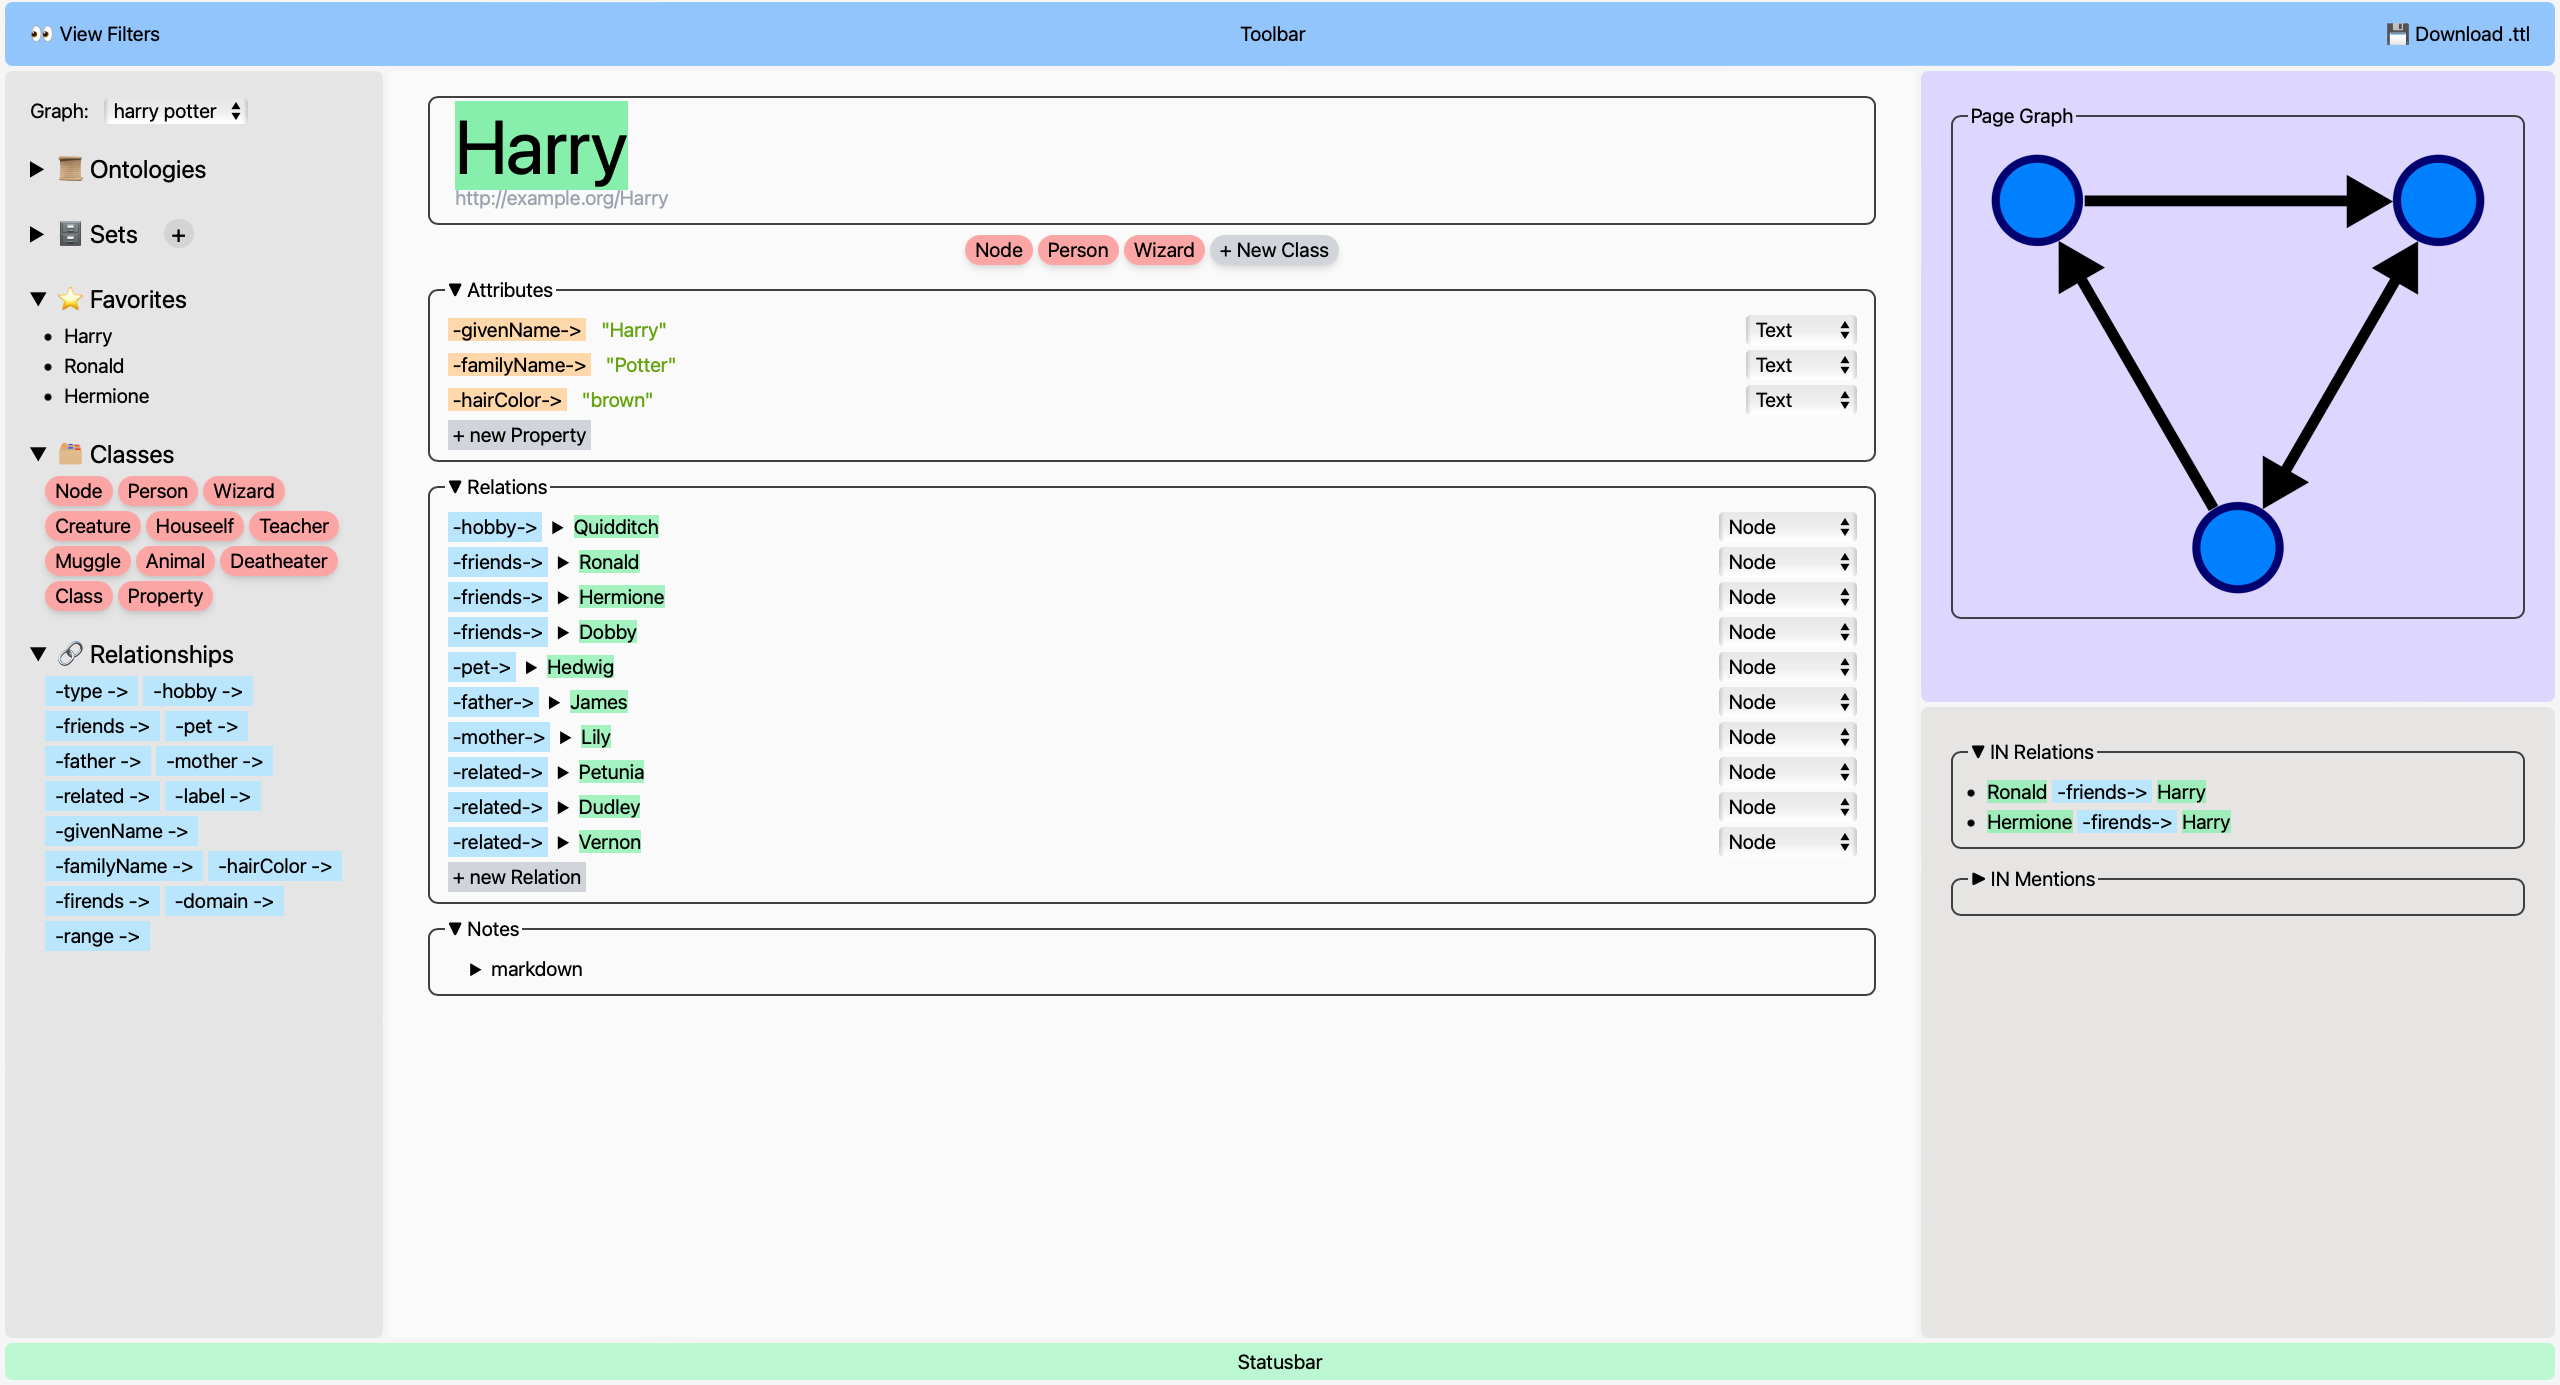
\includegraphics[width=\textwidth]{nink}
\end{figure}

Figure 7.1 shows a screenshot of the UI. It is divided into several Sections, some of them similar to sections found in Apps people frequently use, like note-taking apps, Wikipedia or email clients. From top left to bottom right:
\begin{description}
    \item[Toolbar] The Toolbar is similar to the ones found in modern browsers. It displays open Nodes in Tabs with the IRI appearing as the Title for the Tab. In the outermost corners are shortcuts for accessing prominent functionality.
    \item[Sidebar] The Sidebar serves as navigation and orientation. Users can navigate to Classes, Relationships and their favorite Nodes in the PKG. There are also overviews of used Schema and Sets / Views.
    \item[Editor] The Editor renders all the relevant Information about the currently active Node. The User can toggle which Information is relevant to him and navigate to related Nodes. He can also create, update and delete related Entities and Text.
    \item[Graph panel] The Graph Panel serves as an overview of the context of the current and associated Nodes in visualized form. This provides further orientation and a spatial sense of connectedness in the PKG.
    \item[Relation panel] The Relation Panel shows inferred relations and mentions. (Meaning arcs from other nodes to the current node.
\end{description}

The label and classes of the current node are placed in special positions and hidden from the Relations. The label is prominently displayed as the title, reminiscent of most Text Processors. Classes are presented right below it, similar to tags or categorys in other Applications. This is done to build on the familiarity with similar UIs the User might have interacted with.
    
Notice how Classes, Properties, Entities and Literals are all visually distinguished in the UI, highlighting their different nature and providing easy navigation of the content.

The Semantic Markdown is displayed in a outliner UI, as though it was a hierarchical attachment to the current Node. The structured semantics in it are displayed on the relevant Nodes in an opaque fashion, to hightlight the fact that they are not manifested in the data layer, but rather inferred from Notes. A button enables the user to transform them into explicit statements from the note layer into the data layer. Similar functionality is present for integrating external structured Data (like wikidata, dbpedia, etc.)

\section{Functionality}

The following is an overview of Features and Functionalities of the Prototype.

All of this functionality manipulates the Dataset as outlined in Chapter [Data Model], by creating, updating or deleting RDF triples.
\begin{description}
    \item[Create Node] Pressing the button labeled “+ New Node” in the botton left corner or using the keyboard shortcut “ctrl + n” creates a new Node in the Graph. The User is automatically navigated to the new Node and can edit the Title / Label.
    \item[Attach Class] A new Class can be attached to the current Node by clicking the “+ add Class” button right below the Title / Label.
    \item[Attach Attribute / Relationship] A RDF Triple with the Current Node in subject position can be created by pressing the “+ add Attribute / Relation” Button at the bottom of the respective Sections. This prompts the user to enter a label for the predicate (Relationship) and Object (Target Entity / Literal) of the triple.
    \item[Write Semantic Markdown] In the Notes Section, Semantic Markdown can be edited in an Outliner Text Processor Interface (This feature is not fully implemented yet).
    \item[Switch RDF Graph Dataset] The user can select the RDF Dataset in the “Graph” labeled select input in the Sidebar, to switch between Graph Datasets.
    \item[Import RDF Graphs from URL] The user can import RDF Data from external Sources, by selecting “+ import from URL” from the “Graph” labeled select input in the Sidebar.
\end{description}


\chapter{Discussion} \label{ch:discussion}

use cases:

- government
- public institutions like university and school
    - teachers instead of giving out information about “what” is important,
    - also give out structured information that shows associations
    - this structured knowledge could even be collaboratively maintained across severel schools / universitys

apart from the obvious use cases for personal knowledge graphs, is see the following use cases:

government structured information and databases
government semi-structured information and knowledge, public education

schools and universities
    teaching materials 
    ...

differentiate wikis / PKGs 
pkgs don’t HAVE to be consensus based, but they can.

just like in normal life people with similar ideas will group and build consensus built kgs, like teachings,
\chapter{Conclusions} \label{ch:conclusions}
% This chapter is very generic, it needs to be more specific. 
% What did we accomplish with this thesis? 
% What is left to do? 
% How this can be integrated with SOLID? 

In this thesis, we have investigated PKGs and the PKG ecosystem as approaches to personal knowledge management and the information overload problem. 
We have outlined the functionalities required of the PKG ecosystem and established that PKM tools based on proprietary formats or text files are not viable candidates for the PKG ecosystem. We have proposed RDF as the data model for PKGs and outlined how to store both structured and unstructured data with it. To achieve this we proposed the development of a markdown extension that can express RDF statements. As a proof of concept, we implemented the prototype of a web application that can store structured and unstructured knowledge as an RDF graph.

given more time, we would have developed the prototype with more of a focus on usability by including user tests.

Version control and access rights for PKGs are also topics that we would have liked to investigate in more detail.

Limitations in our approach are that we could not create standards for the RDF data model or semantic markdown. This would require more resources and consensus.

The SOLID project is an initiative by Tim Berners Lee to provide individuals with online data stores, so-called "Pods". These pods could potentially serve as the backend we envisioned for the PKG ecosystem, because they use the RDF data model, and are compatible with several graph query languages \cite{solid}. 


%%%%%%%%%%%%%%%%%%%%%%%%%%%%%%%%%%%%%%%%%%%
% Appendices
%%%%%%%%%%%%%%%%%%%%%%%%%%%%%%%%%%%%%%%%%%%
\appendix
\chapter{The RDFun Javascript Library} \label{apd:rdfun}

RDFun is a JavaScript Library we wrote that implements the RDFJS spec \cite{rdfjs}. 

\lstinputlisting[caption={Dataset.ts}, label=lst:rdfun1]{code/Store.ts}

\newpage
\lstinputlisting[caption=DataFactory.ts, label=lst:rdfun2]{code/DataFactory.ts}



%%%%%%%%%%%%%%%%%%%%%%%%%%%%%%%%%%%%%%%%%%%
% Bibliography
%%%%%%%%%%%%%%%%%%%%%%%%%%%%%%%%%%%%%%%%%%%
\listoffigures 
\begingroup
\let\clearpage\relax
\listoftables
\endgroup
\begingroup
\let\clearpage\relax
\lstlistoflistings
\endgroup
\printbibliography[heading=bibintoc, title={References}]

\end{document}
